%%%%%%%%%%%%%%%%%%%%%%%%%%%%%%%%%%%%%%%%%
% Short Sectioned Assignment LaTeX Template Version 1.0 (5/5/12)
% This template has been downloaded from: http://www.LaTeXTemplates.com
% Original author:  Frits Wenneker (http://www.howtotex.com)
% License: CC BY-NC-SA 3.0 (http://creativecommons.org/licenses/by-nc-sa/3.0/)
%%%%%%%%%%%%%%%%%%%%%%%%%%%%%%%%%%%%%%%%%

%----------------------------------------------------------------------------------------
%	PACKAGES AND OTHER DOCUMENT CONFIGURATIONS
%----------------------------------------------------------------------------------------

\documentclass[paper=a4, fontsize=11pt]{scrartcl} % A4 paper and 11pt font size

% ---- Entrada y salida de texto -----

\usepackage[T1]{fontenc} % Use 8-bit encoding that has 256 glyphs
\usepackage[utf8]{inputenc}
%\usepackage{fourier} % Use the Adobe Utopia font for the document - comment this line to return to the LaTeX default

% ---- Idioma --------

\usepackage[spanish, es-tabla]{babel} % Selecciona el español para palabras introducidas automáticamente, p.ej. "septiembre" en la fecha y especifica que se use la palabra Tabla en vez de Cuadro

% ---- Otros paquetes ----

\usepackage{url} % ,href} %para incluir URLs e hipervínculos dentro del texto (aunque hay que instalar href)
\usepackage{amsmath,amsfonts,amsthm} % Math packages
%\usepackage{graphics,graphicx, floatrow} %para incluir imágenes y notas en las imágenes
\usepackage{graphics,graphicx, float} %para incluir imágenes y colocarlas

% Para hacer tablas comlejas
%\usepackage{multirow}
%\usepackage{threeparttable}

%\usepackage{sectsty} % Allows customizing section commands
%\allsectionsfont{\centering \normalfont\scshape} % Make all sections centered, the default font and small caps

\usepackage{fancyhdr} % Custom headers and footers
\pagestyle{fancyplain} % Makes all pages in the document conform to the custom headers and footers
\fancyhead{} % No page header - if you want one, create it in the same way as the footers below
\fancyfoot[L]{} % Empty left footer
\fancyfoot[C]{} % Empty center footer
\fancyfoot[R]{\thepage} % Page numbering for right footer
\renewcommand{\headrulewidth}{0pt} % Remove header underlines
\renewcommand{\footrulewidth}{0pt} % Remove footer underlines
\setlength{\headheight}{13.6pt} % Customize the height of the header

\numberwithin{equation}{section} % Number equations within sections (i.e. 1.1, 1.2, 2.1, 2.2 instead of 1, 2, 3, 4)
\numberwithin{figure}{section} % Number figures within sections (i.e. 1.1, 1.2, 2.1, 2.2 instead of 1, 2, 3, 4)
\numberwithin{table}{section} % Number tables within sections (i.e. 1.1, 1.2, 2.1, 2.2 instead of 1, 2, 3, 4)

\setlength\parindent{0pt} % Removes all indentation from paragraphs - comment this line for an assignment with lots of text

\newcommand{\horrule}[1]{\rule{\linewidth}{#1}} % Create horizontal rule command with 1 argument of height


%----------------------------------------------------------------------------------------
%	TÍTULO Y DATOS DEL ALUMNO
%----------------------------------------------------------------------------------------
\usepackage[sfdefault]{roboto}
\usepackage{sectsty}
\usepackage{hyperref}


\sectionfont{\fontsize{12}{15}\selectfont}
\title{	
\normalfont \normalsize 
\textsc{\textbf{Ingeniería de Servidores (2016-2017)} \\ Grado en Ingeniería Informática \\ Universidad de Granada} \\ [25pt] % Your university, school and/or department name(s)
\horrule{0.5pt} \\[0.4cm] % Thin top horizontal rule
\huge Memoria Práctica 1 \\ % The assignment title
\horrule{2pt} \\[0.5cm] % Thick bottom horizontal rule
}

\author{Sergio Cervilla Ortega} % Nombre y apellidos

\date{\normalsize\today} % Incluye la fecha actual

%----------------------------------------------------------------------------------------
% DOCUMENTO
%----------------------------------------------------------------------------------------

\begin{document}

\maketitle % Muestra el Título

\newpage %inserta un salto de página

\tableofcontents % para generar el índice de contenidos

\listoffigures

\listoftables

\newpage

%----------------------------------------------------------------------------------------
%	CUESTIÓN 1
%----------------------------------------------------------------------------------------
\section{¿Qué modos y/o tipos de virtualización existen?}

Un buen criterio a la hora de virtualizar es según la cantidad de hardware virtualizado. Esto es muy interesante y creo que es uno de los puntos fuertes del software dedicado a la virtualización ya que permite virtualizar desde todo el hardware subyacente a la máquina a tan solo una pequeña porción. Esto puede resultar muy interesante ya que podemos comprobar la utilización de los recursos físicos por parte de la máquina virtual, en el sentido de que podemos comprobar como funcionaría un cierto software o cierto sistema simulando una máquina antigua, lo cual lo podemos conseguir asignando pocos cores y poca RAM.\\

Está claro que para lograr un mejor rendimiento en lo previamente mencionado deberíamos de virtualizar apoyándonos en el hardware ya que así ciertas instrucciones se ejecutarían directamente en el procesador físico, consiguiendo un rendimiento más cercano a la realidad, pero, por otro lado, tenemos la virtualización por software, en la cual tendríamos que simular también el hardware y por tanto el rendimiento podría ser bastante inferior al esperado.




%----------------------------------------------------------------------------------------
%	CUESTIÓN 2
%----------------------------------------------------------------------------------------
\section{Muestre los precios y características de varios proveedores de VPS (Virtual Private Server) y compare con el precio de servidores dedicados (administrados y no administrados). Comente las diferencias.}
Primero he comprobado los precios en la web dinahosting.com \cite{dinahosting} y la tabla de precios aproximada es la siguiente:

\begin{table}[H]
	\centering
	\begin{tabular}{|c|c|c|}
		\hline
		\textbf{ } & \textbf{Administrado} & \textbf{No Administrado} \\
		\hline
		Dedicado & 2045€/año & 1525€/año \\
		Virtual & 509€/año & 422€/año \\
		\hline
	\end{tabular}  
	\caption{Tabla de precios de servidores en dinahosting.com.} \label{tab:tablasencilla}
\end{table}

Para esta tabla hemos utilizado los planes que ofrecen unas características medias para lograr un buen equilibrio entre calidad/precio. En concreto, para el servidor dedicado he utilizado, tanto para la modalidad administrada como no administrada, el modelo Dell PowerEdge R230 con las siguientes características:
\begin{itemize}
	\item DELL R230 con procesador Intel® Xeon® processor E3-1230 v5.
	\item 4GB de RAM.
	\item 1TB de espacio.
	\item 100Mbit/s de conectividad.
\end{itemize}


 y para el Servidor Privado Virtual, administrado y no administrado, las siguientes características:
 \begin{itemize}
 	\item 1 VCPU, SAS.
 	\item 1,5GB de RAM.
 	\item 30GB de espacio.
 	\item 1TB de tráfico.
 \end{itemize} 


Para contrastar un poco los precios he consultado 1and1 \cite{1and1} también, la cual nos ofrece los siguientes precios para servidores dedicados y VPS:
\begin{table}[H]
	\centering
	\begin{tabular}{|c|c|c|}
		\hline
		\textbf{ } & \textbf{Administrado} & \textbf{No Administrado} \\
		\hline
		Dedicado & 2160€/año & 1980€/año \\
		Virtual & 180€/año & 70€/año \\
		\hline
	\end{tabular}  
	\caption{Tabla de precios de servidores en 1and1.es.} \label{tab:tablasencilla}
\end{table}

Las características del servidor dedicado son las siguientes: 
\begin{itemize}
	\item Procesador AMD Opteron™ 6338P con 12 Cores x 2,3 GHz.
	\item 32 GB DDR3 ECC
	\item 2TB de espacio.
	\item Software RAID1
\end{itemize}

Las características del VPS son las siguientes:
\begin{itemize}
	\item 1 vCore Procesadores Intel® Xeon®.
	\item 1Hb de RAM
	\item 50GB de SSD.
\end{itemize}

%----------------------------------------------------------------------------------------
%	CUESTIÓN 3
%----------------------------------------------------------------------------------------

\section{a) Enumere y explique brevemente al menos tres de las innovaciones en Windows Server 2016 y 2012 R2 respecto a 2008 R2.\newline b)¿Qué es Windows Server 2016 nano? }

\textbf{a)} Una innovación respecto al sistema que hubo en Windows Server 2012 R2 en comparación con Windows Server 2008 R2 y que a mi parecer puede ser de las más importantes es respecto a las máquinas virtuales \cite{microsoftmv}, ya que la versión del 2008 podía mantener activas hasta 384 pero en la versión de 2012 el salto fue gigantesco ya que en este caso se pueden mantener hasta 1024 máquinas simultáneas. \\



Además, respecto al almacenamiento, Windows Server 2012 R2 permite un espacio de almacenamiento con niveles \cite{seagatelevels}. Esto significa que ya no todo tiene que ser almacenar información en HDD's simples, que aunque ejercen su función, pueden llegar a ocasionar cuellos de botella, sino que ahora se han creado varios niveles dentro de esta funcionalidad, siendo más personalizable y pudiendo aumentar en una cantidad significativa el rendimiento de nuestros servidores mediante el uso, por ejemplo, de unidades SSD.\\




Por último, comentar también una última mejora respecto a las virtualizaciones de redes, en concreto, la versión de 2012 incluyó la virtualización de red de Hyper-V \cite{hyperV}. Este tipo de virtualización permite a los clientes ser "propietarios" de un conjunto de máquinas virtuales, o red de máquinas virtuales  implementadas en un centro de datos. \\

 
\textbf{b)} Windows Server 2016 Nano \cite{wnano} se podría decir que es una instalación minimalista de Windows Server ya que tan solo instala la PowerShell, por lo tanto, es un sistema muchísimo más ligero que las otras versiones. Además, Windows Server 2016 Nano está preparado de forma nativa para trabajar sobre la nube.


%----------------------------------------------------------------------------------------
%	CUESTIÓN 4
%----------------------------------------------------------------------------------------
\section{¿Qué son los productos MAAS y Landscape ofrecidos por Canonical (la empresa que desarrolla Ubuntu)?}
MAAS \cite{MAAS} significa Metal As A Service y es un servicio que permite tratar un conjunto de servidores físicos como un conjunto de máquinas virtuales en la nube, consiguiendo de esta manera un servicio mucho más flexible ya que además de ser un servicio autónomo tiene la posibilidad de ser utilizado junto a otras tecnologías, como puede ser Juju. \\


Landscape \cite{Landscape} es una herramienta de gestión de sistemas cuya utilidad reside en la posibilidad de administrar un gran número de máquinas desde una sola. Gracias a la posibilidad de agrupar un gran número de máquinas bajo una etiqueta es muy sencillo realizar cambios en grupos de instancias muy bien definidos. Además, Landscape ofrece la posibilidad de crear scripts, que sumado a la posibilidad de crear grupos de máquinas, ofrece un servicio con un gran potencial.


%----------------------------------------------------------------------------------------
%	CUESTIÓN 5
%----------------------------------------------------------------------------------------
\section{¿Qué relación tiene esta distribución (CentOS) con Red Hat y con el proyecto Fedora?}
CentOS \cite{centOS} es un sistema cuyo mantenimiento depende de la comunidad, está basado en código abierto liberado por Red Hat, Inc. \cite{RedHat} y es básicamente la versión de la comunidad de RedHat.  
Fedora \cite{Fedora} es el proyecto principal y es una distribución de código abierto, gratuita y Community Driven.
Red Hat Enterprise Linux (RHEL) \cite{RHEL} es la versión de pago de Fedora, y por tanto tiene soporte oficial y lanzamientos de nuevas versiones más lentos pero mejor desarrollados ya que han sido supervisados previamente. \\ 

La dependencia entre estos sistemas es la siguiente:
Primero RedHat creó el proyecto Fedora y de éste nació el sistema RHEL, que como dije anteriormente, es la versión de pago de Fedora, con todas las ventajas que esto conlleva. Por último, surgió CentOS, que es un sistema que utiliza el código ya liberado por RHELL.


%----------------------------------------------------------------------------------------
%	CUESTIÓN 6
%----------------------------------------------------------------------------------------
\section{¿Qué diferencias hay entre RAID mediante software y mediante hardware?}
Un RAID basado en hardware es completamente independiente de la máquina que lo vaya a utilizar y se le presenta a la misma como una única entidad aunque físicamente esté formada por varios discos. El problema de este tipo de RAIDs es el precio de los controladores necesarios que se encargan de gestionar el RAID para liberar a la CPU de esa carga, ya que se deben de conectar a un controlador SCSI que unifica varios discos para presentarle a la máquina host que es tan solo uno. \\

Sin embargo, un RAID software ofrece una solución a un coste menor y además puede ofrecer un mejor rendimiento ya que éste depende directamente de la potencia y/o rendimiento de la CPU aunque si esta se satura, se reducirá gravemente el rendimiento. Los RAID basados en software tienen la ventaja de que en un único disco físico podemos establecer varios dispositivos de bloque y mostrárselo al sistema como uno solo. \\

Información obtenida de Massachusetts Institute of Technology \cite{mitraid}.


%----------------------------------------------------------------------------------------
%	CUESTIÓN 7
%----------------------------------------------------------------------------------------
\section{a) ¿Qué es LVM? \newline b) ¿Qué ventaja tiene para un servidor de gama baja? \newline  c) Si va a tener un servidor web, ¿le daría un tamaño grande o pequeño a /var?}
\textbf{a)} LVM \cite{LVM} es, como su propio nombre indica, un Logical Volume Manager, que traducido al español sería un administrador de volúmenes lógicos. Tiene 3 elementos clave:\\
\begin{itemize}
	\item Logical Volume: Es parecido a una partición y por tanto puede contener sistemas de archivos. En esta práctica tendremos 4 (/, /home, /boot y /swap).
	\item Logical Volume Group: Es parecido a un disco duro y hasta que no se añada un PV no podemos utilizarlo.
	\item Physical Volumes: Son las particiones del disco duro y puede ser un RAID.
\end{itemize}


\textbf{b)} La principal ventaja en servidores de gama baja \cite{lvmlowcost} es que al no disponer de una gran cantidad de recursos como para poder despreocuparnos de que se llenen los discos, LVM puede redimensionarlos dinámicamente y asignarle más espacio a otra de las particiones. Por ejemplo, si hemos llenado /home pero tenemos mucho espacio sin utilizar en otra partición, como por ejemplo, /, LVM se encarga de asignarle este espacio a /home reduciendo el tamaño de / pero sin pérdida de datos en ninguna de ellas. La única restricción es que todos tienen que permanecer al mismo LVG y que el sistema de ficheros soporte el redimensionamiento por arriba y por abajo.\\

\textbf{c)} Le deberíamos de dar un tamaño algo más grande que a otras particiones ya que esta es una partición que va creciendo dinámicamente y por tanto es aconsejable que no se quede sin espacio \cite{var}. Además como en esta partición se almacenan todas las variables del sistema, incluidas algunas temporales, es mejor asignarle un tamaño más grande.


%----------------------------------------------------------------------------------------
%	CUESTIÓN 8
%----------------------------------------------------------------------------------------
\section{¿Debemos cifrar también el volumen que contiene el espacio para swap? ¿y el volumen en el que montaremos /boot?}
Debemos de cifrar todos los volúmenes que puedan contener información sensible. En este caso, sí deberíamos de cifrar swap ya que al utilizarse como espacio de intercambio, no sabemos que tipo de información puede acabar ahí almacenada y por tanto si no estuviera cifrada alguien podría acceder a esta y con un poco de suerte para él, y mala suerte para nosotros, puede dar con diversas contraseñas o información que no deseamos que salga de nuestro disco. \\

Sin embargo, /boot no contienen ningún tipo de información sensible ya que tan solo contiene información del arranque y no tendría ningún sentido cifrarlo.

%----------------------------------------------------------------------------------------
%	CUESTIÓN 9
%----------------------------------------------------------------------------------------
\section{a) Imagine que tiene un disco híbrido con tecnología SSD. ¿Qué puntos de montaje ubicaría en este? \newline b) Justifique qué tipo de sistema de archivos usaría para tener un servidor de streaming.}
\textbf{a)} Debido a que los SSD tienen un número limitado de escrituras pero no de lecturas, se deberían de almacenar aquellas particiones en las que se escriba en una menor cantidad y con una menos frecuencia, estos serían:
\begin{itemize}
	\item /
	\item /boot
	\item /usr
\end{itemize}
Y en el HDD, debido a que este no tiene esa limitación, pondríamos: 
\begin{itemize}
	\item /home
	\item /swap
	\item /tmp
\end{itemize}

\textbf{b)} Utilizaría el sistema de archivos NFS \cite{NFS}, que además de ser eso, un sistema de archivos, es un protocolo el cual nos facilita la compartición de archivos a través de la red, permitiendo a los clientes acceder a estos recursos como si fuera de manera local, cuando en realidad están accediendo a un sistema de archivos remoto. Como lo que queremos crear es un servidor de streaming este sistema de archivos es bastante bueno ya que nos facilita la compartición de los datos.

%----------------------------------------------------------------------------------------
%	CUESTIÓN 10
%----------------------------------------------------------------------------------------
\section{Muestre cómo ha quedado el disco particionado una vez el sistema está instalado y ha iniciado sesión.}

\begin{figure}[H]
	\centering
	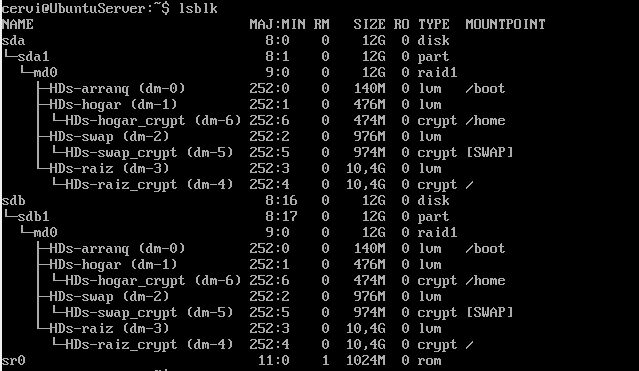
\includegraphics[scale=0.75]{lsblk.png}
	\caption{Resultado de ejecutar \textbf{lsblk} en mi terminal después de montar el sistema. \label{fig:figura1}}
\end{figure}


%----------------------------------------------------------------------------------------
%	CUESTIÓN 11
%----------------------------------------------------------------------------------------
\section{a) ¿Cómo ha hecho el disco 2 ``arrancable''? \newline b) ¿Qué hace el comando grub-install?}
\textbf{a)} Para solucionar el bug de arranque del disco 2 tenemos que esperar a que aparezca la consola auxiliar \textbf{initrams}. Una vez la tenemos, podemos comprobar que haciendo \textit{cat /proc/mdstat} el RAID está marcado como inactive, y este bug hace que a pesar de que realmente esté degradado se marque como inactivo y no podamos arrancar. Para lograrlo tenemos que utilizar \textit{mdstat -R /dev/md0} para forzar a los discos a estar activos y por último ejecutar \textit{exit} para salir de initrams. Podemos comprobar entonces que ya se nos pide la clave de cifrado y podemos arrancar el sistema con normalidad. \\

\textbf{b)} El comando instala grub \cite{grub} en un disco el cual debemos indicar después del comando, como por ejemplo \textit{grub-install /dev/sda}

%----------------------------------------------------------------------------------------
%	CUESTIÓN 12
%----------------------------------------------------------------------------------------
\section{¿Qué diferencia hay entre Standard y Datacenter?}
Ambas versiones ofrecen toda la funcionalidad de Windows Server pero la principal diferencia está en que la versión standard permite la virtualización de como máximo 2 instancias virtuales mientras que la versión datacenter no está limitada a un número concreto de instancias.

La comparación completa la podemos encontrar en la página oficial \cite{windows_std_data}.



%----------------------------------------------------------------------------------------
%	CUESTIÓN 13
%----------------------------------------------------------------------------------------
\section{Continúe usted con el proceso de definición de RAID1 para los dos discos de 50MiB que ha creado. Muestre el proceso con capturas de pantalla.}

Una vez añadidos los discos lo único que tenemos que hacer es click derecho en propiedades y pulsar sobre \textit{New Mirrored Volume}. Avanzamos hasta la siguiente parte donde nos salen los dos discos, o más en caso de tenerlos y lo único que tenemos que hacer es pulsar sobre el de la izquierda y darle a añadir. El siguiente paso consiste en asignarle una etiqueta si es que queremos además de la opción de un formateo rápido y al seguir avanzando finalizamos el proceso de manera natural.

\begin{figure}[H]
	\centering
	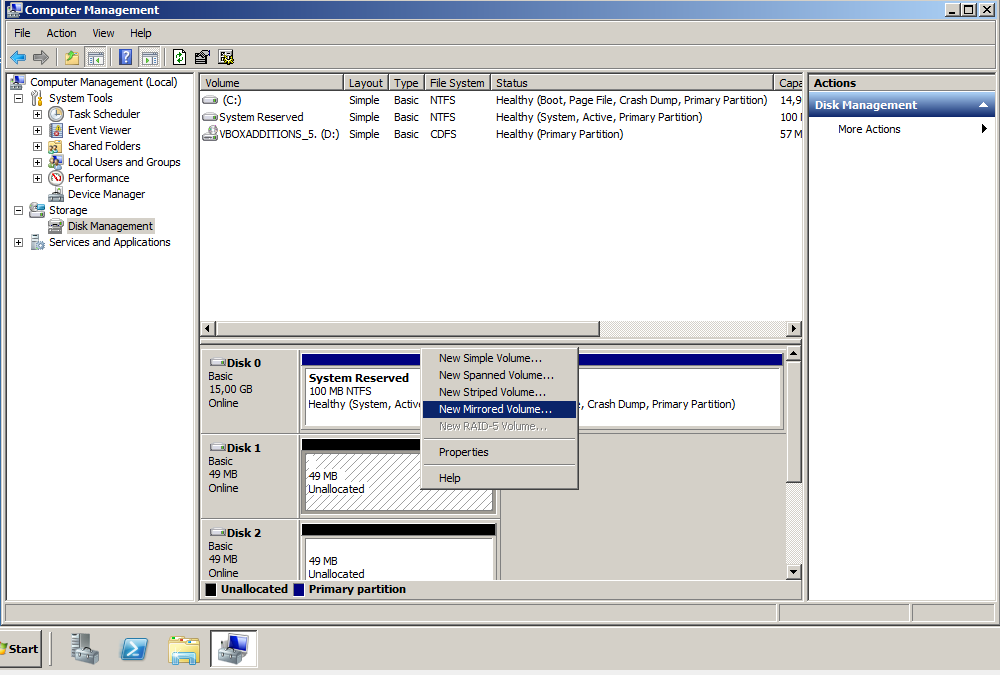
\includegraphics[scale=0.45]{RAIDW1.png}
	\caption{Primer paso RAID Windows. \label{fig:figura5}}
\end{figure}

\begin{figure}[H]
	\centering
	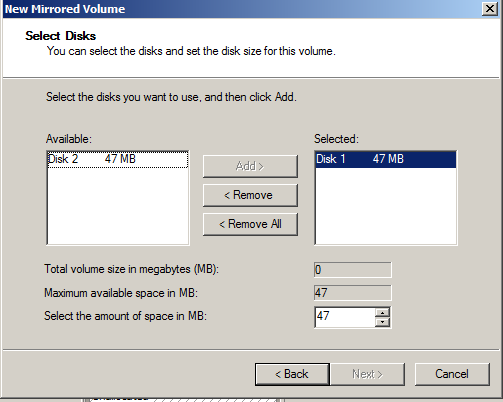
\includegraphics[scale=0.75]{RAIDW2.png}
	\caption{Segundo paso RAID Windows. \label{fig:figura6}}
\end{figure}

\begin{figure}[H]
	\centering
	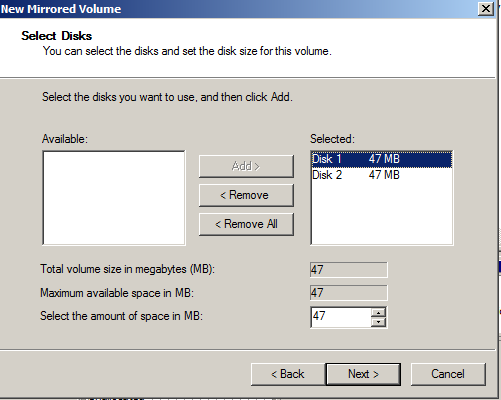
\includegraphics[scale=0.75]{RAIDW3.png}
	\caption{Tercer paso RAID Windows. \label{fig:figura7}}
\end{figure}

\begin{figure}[H]
	\centering
	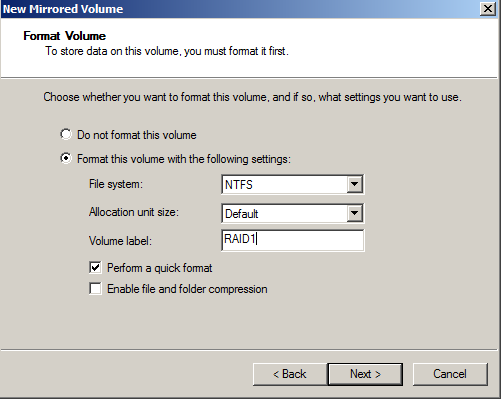
\includegraphics[scale=0.75]{RAIDW4.png}
	\caption{Cuarto paso RAID Windows. \label{fig:figura8}}
\end{figure}

\begin{figure}[H]
	\centering
	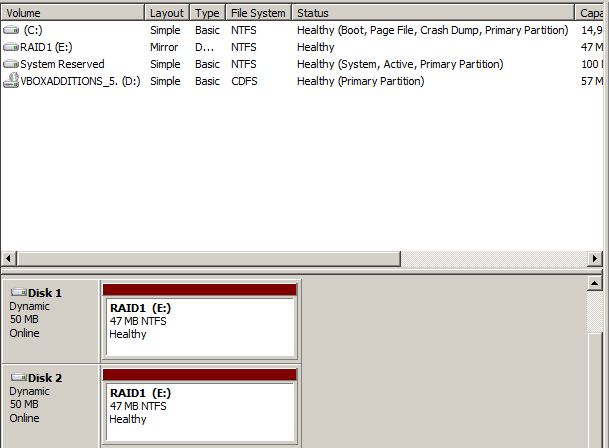
\includegraphics[scale=0.65]{RAIDW5.png}
	\caption{RAID en Windows operativo. \label{fig:figura9}}
\end{figure}

%----------------------------------------------------------------------------------------
%	CUESTIÓN 14
%----------------------------------------------------------------------------------------
\section{Explique brevemente qué diferencias hay entre los tres tipos de conexión que permite el VMSW para las Mvs: NAT, Host-only y Bridge.}

\begin{itemize}
	\item \textbf{NAT:} Debido a que es la opción más sencilla de conectividad entre una máquina virtual y una red es la opción por defecto de VirtualBox. Este tipo de conexión hace que el propio VirtualBox actúe como router, asignando direcciones IP completamente diferentes a las de la máquina host a las máquinas virtuales y además como es tratada como una red separada la máquina host no puede acceder a ninguna de las máquinas guest.
		\begin{figure}[H]
			\centering
			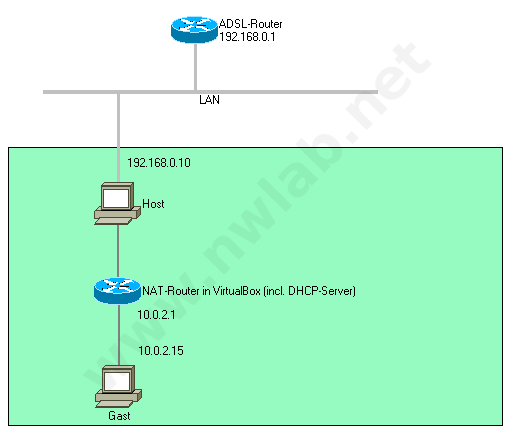
\includegraphics[scale=0.5]{nat-virtualbox.png}
			\caption{Configuración NAT en VirtualBox.\cite{figura141} \label{fig:figura2}}
		\end{figure}
	\item \textbf{Bridge:} En esta configuración tanto la máquina host como la guest, utilizan el mismo adaptador de red y por tanto es como si ambas máquinas estuvieran conectadas físicamente con un cable de red.
		\begin{figure}[H]
			\centering
			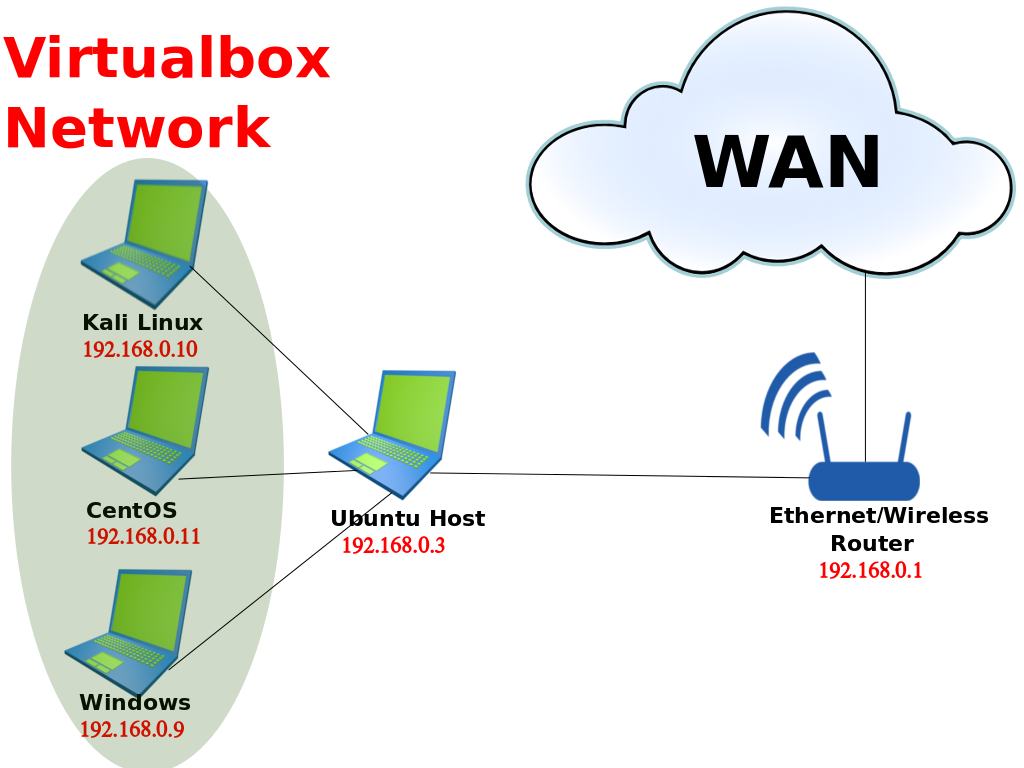
\includegraphics[scale=0.24]{bridge-virtualbox.png}
			\caption{Configuración Bridge en VirtualBox.\cite{figura142} \label{fig:figura3}}
		\end{figure}
	\item \textbf{Host-only:} En esta configuración es prácticamente un híbrido entre NAT y Bridge ya que las máquinas se pueden comunicar entre ellas, tanto host como guest y además se crea un nuevo interfaz software.
		\begin{figure}[H]
			\centering
			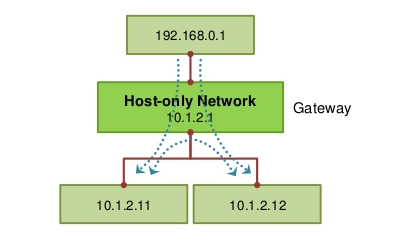
\includegraphics[scale=0.9]{host-only-virtualbox.png}
			\caption{Configuración Host-only en VirtualBox.\cite{figura143} \label{fig:figura4}}
		\end{figure}
\end{itemize}

Toda la información ha sido obtenida del capítulo 6 del manual de VirtualBox, excepto las imágenes ilustrativas. 



\bibliography{citas} %archivo citas.bib que contiene las entradas 
\bibliographystyle{plain} % hay varias formas de citar
\end{document}
